\documentclass[a4paper]{article}
\usepackage{authblk}
\usepackage[font=small,labelfont=bf]{caption}
\usepackage{biblatex}
\addbibresource{references.bib}
\usepackage{lineno}
\usepackage{amsmath}
\usepackage{amsfonts}
\usepackage{tikz}
\usepackage{tkz-graph}
\usepackage{mathtools}
\usepackage{tabularx}
\usepackage{graphicx}
\usepackage{blkarray}
\usepackage{booktabs} 
\graphicspath{ {./figures/} }


\title{Optimal threshold problem: A novel 0-1 ILP-based approach}
\date{}
\author[1]{Pouria Ramazi}
\author[2]{Arash Mari Oriyad}
\affil[1]{Department of Mathematics and Statistics, Brock University, St. Catharines, L2S 3A1, ON, Canada}
\affil[2]{Department of Electrical and Computer Engineering, Isfahan University of Technology, Isfahan 84156-83111, Iran}
\setcounter{Maxaffil}{0}
\renewcommand\Affilfont{\small}

\usepackage[utf8]{inputenc}
\usepackage{fourier, heuristica}
\usepackage[colorlinks=true]{hyperref}
\usepackage{array, ltablex, multirow}

\usepackage{makecell}
\setcellgapes{5pt}
\makegapedcells
\renewcommand\theadfont{\bfseries}
\renewcommand\cellalign{rc}


\begin{document}
\maketitle
%\linenumbers


%\begin{abstract}
%Abstract ... 
%\end{abstract}

Accuracy \cite{accuracy}, recall \cite{recall}, specificity \cite{specificity}, and precision are four of the most commonly-used performance measures to evaluate binary classification models. Considering $TP$, $TN$, $FP$, and $FN$ as the number of true-positive, true-negative, false-positive, and false-negative instances, respectively, these measures are defined as follows:

\begin{equation}
\label{definition}
\begin{aligned}
&accuracy = \frac{TP + TN}{TP + TN + FP + FN}\\
&recall = \frac{TP}{TP + FN}\\
&specificity=\frac{TN}{TN + FP}\\
&precision= \frac{TP}{TP + FP}\\
\end{aligned}
\end{equation}

While calculating performance measures introduced in equation \ref{definition} require deterministic labels, classification models often produce probabilistic outputs. Hence, one must apply a threshold to the probabilities generated by a classifier to obtain deterministic labels. An optimal accuracy (resp. recall, specificity, and precision) threshold for a given set of instances is a real value between 0 and 1, resulting in the highest accuracy (resp. recall, specificity, and precision).

A trivial approach to determine such a threshold is an exhaustive search over all possible thresholds to obtain the best one. As an alternative method, we introduce a 0-1 integer linear programming (ILP) formulation to the problem of finding the optimal threshold for accuracy, recall, specificity, precision, and any linear combination of them.

Assume a set of $N$ instances with a binary target variable $y$. We call $N^+$ and $N^-$ as the number of positive and negative instances. Also, suppose $\hat{y_i}$ is the probability generated by a binary classifier for the $i$th instance. Then, $\tilde{y_i}$ would be a binary decision variable that represents the label of $i$th instance after applying the threshold $\tau$ to $\hat{y_i}$. More precisely, if $\hat{y_i} < \tau$, then $\tilde{y_i}$ will be $0$ and vice versa. The goal is to find a value for $\tau$ which maximize a linear function of performance measures.

Using the introduced notations and according to equation \ref{definition}, accuracy, recall, specificity, and precision can be calculated as follows:

\begin{equation}
\begin{aligned}
&accuracy = 1 - \frac{1}{N} \sum_{i=1}^{N} |y_i - \tilde{y_i}|\\
&recall = \frac{1}{N^+} \sum_{i=1}^{N} y_i \tilde{y_i}\\
&specificity = \frac{1}{N^-} \sum_{i=1}^{N} (1-y_i) (1-\tilde{y_i})\\
&precision = \frac{\sum_{i=1}^{N} y_i \tilde{y_i}}{\sum_{i=1}^{N} \tilde{y_i}}\\
\end{aligned}
\end{equation}

Put them all together, the following optimization formulation is achieved to find the optimal threshold maximizing $\alpha \times \textit{accuracy} + \beta \times \textit{recall} + \gamma \times \textit{specificity} + \zeta \times precision$, where $\alpha$, $\beta$, $\gamma$, and $\zeta$ are arbitrary coefficients set by user.

\begin{equation}
\label{optimization_formulation}
\begin{aligned}
	&\text{maximize} \quad \sum_{i=1}^{N} \left(-\frac{\alpha}{N}|y_i -\tilde{y_i}| + \frac{\beta}{N^+} y_i \tilde{y_i} + \frac{\gamma}{N^-} (1-y_i) (1-\tilde{y_i})\right) + \zeta \frac{\sum_{i=1}^{N} y_i \tilde{y_i}}{\sum_{i=1}^{N} \tilde{y_i}}\\
	&\text{subject to:} \quad \tilde{y_i} = 
	\begin{cases}
	0, & \hat{y_i} < \tau \\
	1, & \hat{y_i} \ge \tau
	\end{cases} \qquad \forall 1\le i \le N\\
	& \qquad \qquad \qquad \tilde{y_i} \in \{0, 1\} \qquad \forall 1\le i \le N\\
	& \qquad \qquad \qquad 0 \le \tau \le 1 \qquad
\end{aligned}
\end{equation}

To make the term $|y_i -\tilde{y_i}|$ linear, we introduced new decision variable $z_i$ along with 2 new constraints for each $i$ shown in equation \ref{ilp}. More precisely, constraints $(1)$ and $(2)$ force the decision variable $z_i$ to be greater than $|y_i - \tilde{y_i}|$, and hence, by maximizing $-z_i$, we are maximizing $-|y_i - \tilde{y_i}|$ too.

Linearizing the term $\frac{\sum_{i=1}^{N} y_i \tilde{y_i}}{\sum_{i=1}^{N} \tilde{y_i}}$ ...

 Moreover, to linearize $\tilde{y_i}$ constraints in equation \ref{optimization_formulation}, we combined the conditions and replace them with two new constraint sets $(3)$ and $(4)$ for each $i$ in equation \ref{ilp}. These constraints are formulating the relation between $\tilde{y_i}$ and $\tau$. For example, if $\hat{y_i} = 0.7$ and $\tau=0.5$ for an arbitrary $i$, then $\tilde{y_i}$ is forced to be $1$ according to the constraints $0.7 (1 - \tilde{y_i}) < 0.6$ and $\tilde{y_i} (0.7 - 1) \ge 0.6 - 1$.

\begin{equation}
\label{ilp}
\begin{aligned}
&\text{maximize} \quad \sum_{i=1}^{N} \left(-\frac{\alpha}{N}|y_i -\tilde{y_i}| + \frac{\beta}{N^+} y_i \tilde{y_i} + \frac{\gamma}{N^-} (1-y_i) (1-\tilde{y_i})\right) + \zeta \frac{\sum_{i=1}^{N} y_i \tilde{y_i}}{\sum_{i=1}^{N} \tilde{y_i}}\\
&\text{subject to:}\\
&\quad \: \: z_i \ge y_i - \tilde{y_i} \qquad \forall 1\le i \le N \qquad (1)\\
& \quad z_i \ge \tilde{y_i}  - y_i \qquad \forall 1\le i \le N \qquad (2)\\
& \quad \hat{y_i} (1 - \tilde{y_i}) < \tau \qquad \forall 1\le i \le N \qquad (3)\\
& \quad  \tilde{y_i} (\hat{y_i} - 1) \ge \tau - 1 \qquad \forall 1\le i \le N \qquad (4)\\
& \quad \tilde{y_i} \in \{0, 1\} \qquad \forall 1\le i \le N \\
& \quad z_i \in \mathbb{R} \qquad \forall 1\le i \le N \\
& \quad  0 \le \tau \le 1
\end{aligned}
\end{equation}

Note that the proposed ILP formulation in equation \ref{ilp} cannot output $t=0$ as the optimal threshold and this case must be considered separately. 

To further improve the ILP formulation, we considered a case where number of unique ordered pairs $(y_i,\: \hat{y_i})$ for $1 \le i \le N$ is significantly less than total number of instances, $N$. Suppose $M$ is the total number of distinct ordered pairs, and $m_i$ is the repetition number of a particular ordered pair in the original instance set. Hence, the following ILP formulation is equivalence to the previous one but empirically more efficient when $M << N$.

\begin{equation}
\label{improved_ilp}
\begin{aligned}
&\text{maximize} \quad \sum_{i=1}^{M} m_i \left(-\frac{\alpha}{N}|y_i -\tilde{y_i}| + \frac{\beta}{N^+} y_i \tilde{y_i} + \frac{\gamma}{N^-} (1-y_i) (1-\tilde{y_i})\right) + \zeta \frac{\sum_{i=1}^{M} m_i y_i \tilde{y_i}}{\sum_{i=1}^{M} m_i \tilde{y_i}}\\
&\text{subject to:}\\
&\quad \: \: z_i \ge y_i - \tilde{y_i} \qquad \forall 1\le i \le M \qquad\\
& \quad z_i \ge \tilde{y_i}  - y_i \qquad \forall 1\le i \le M \qquad\\
& \quad \hat{y_i} (1 - \tilde{y_i}) < \tau \qquad \forall 1\le i \le M \qquad\\
& \quad  \tilde{y_i} (\hat{y_i} - 1) \ge \tau - 1 \qquad \forall 1\le i \le M \qquad\\
& \quad \tilde{y_i} \in \{0, 1\} \qquad \forall 1\le i \le M \\
& \quad z_i \in \mathbb{R} \qquad \forall 1\le i \le M \\
& \quad  0 \le \tau \le 1
\end{aligned}
\end{equation}

The proposed ILP-based approach is compared with a simple exhaustive search method with time complexity of $O(N^2)$ in terms of average execution time where $\alpha=1$, $\beta=0$, $\gamma=0$, and $\zeta=0$ (Fig. 1).

\begin{figure}[t]
	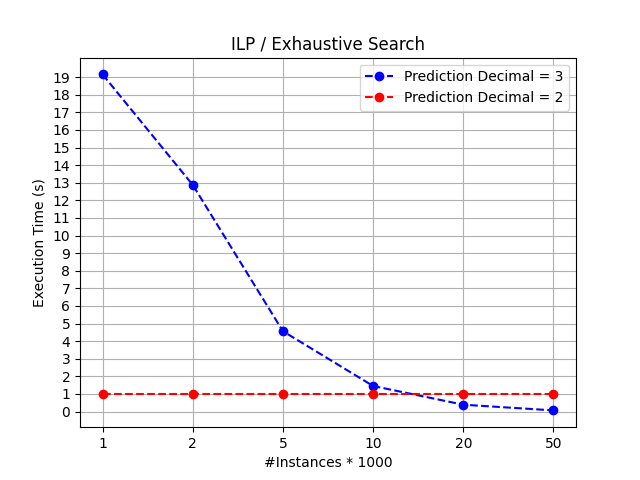
\includegraphics[width=\columnwidth]{figure_4_temp}
	\caption{Comparison between ILP and exhaustive search methods in terms of average execution time. Each curve demonstrates the proportion of obtained average execution time by the ILP approach respect to the search method. All experiments were repeated 100 times and predictions were generated using the continuous uniform distribution $U[0, 1]$.}
\end{figure}

Results demonstrate that by increasing the number of instances ($N$), the ILP method eventually overcomes the exhaustive search.  

\printbibliography

\end{document}
